\chapter{Architecture et Choix Techniques}

Pour répondre aux exigences de maintenabilité et de simplicité de déploiement imposées par le sujet [cite: 12, 14], nous avons fait le choix de nous écarter des solutions CMS existantes pour développer une application sur mesure[cite: 11]. Nos choix technologiques ont été guidés par deux critères majeurs : la robustesse de la solution et notre volonté de consolider des compétences demandées dans le monde de l'entreprise.

\section[Frontend : Angular]{Frontend : Angular \raisebox{-0.2\height}{
\includegraphics[height=0.6cm]{img/logo_angular.jpeg}}}
Pour l'interface utilisateur, notre choix s'est porté sur le framework Angular. Ce choix s'explique tout d'abord par une compétence déjà présente au sein de l'équipe (deux membres avaient déjà utilisé cette technologie). De plus, Angular est aujourd'hui un standard de l'industrie pour les applications web complexes (Single Page Applications). Sa structure basée sur les composants et l'utilisation de TypeScript garantissent un code typé, maintenable et évolutif.

\section[Backend : Node.js]{Backend : Node.js \raisebox{-0.2\height}{
\includegraphics[height=0.6cm]{img/logo_nodejs.png}}}
Bien que notre formation de 5 ans en informatique nous ait permis d'acquérir une grande expertise sur le langage comme Java, nous avons décidé d'implémenter notre API Backend en Node.js. Ce choix est doublement stratégique. D'une part, Node.js est extrêmement populaire dans l'industrie actuelle pour le développement de micro-services et d'API REST. D'autre part, cela nous permettait de sortir de notre zone de confort académique (Java) pour relever un défi technique pertinent pour notre future insertion professionnelle.

\section[Base de données : PostgreSQL]{Base de données : PostgreSQL \raisebox{-0.2\height}{
\includegraphics[height=0.6cm]{img/logo_postgresql.jpeg}}}
Le système devant gérer de potentielles écritures simultanées (modification de salles, ajout de matériels), nous avons rapidement écarté SQLite. Très léger, SQLite nous semblait trop faible pour nos besoins. Notre choix final s'est donc porté sur PostgreSQL, un Système de Gestion de Base de Données Relationnelle (SGBDR) robuste et open-source. Il s'intègre également de manière fluide avec Node.js.

\subsection{Schéma de fonctionnement}
Le schéma suivant illustre le workflow principal de l'application : l'utilisateur interagit avec le frontend Angular, qui transmet des requêtes HTTP au backend Node.js. Ce backend traite la logique métier, interroge PostgreSQL pour lire ou modifier les données, puis renvoie les réponses au frontend.

\begin{figure}[h]
    \centering
    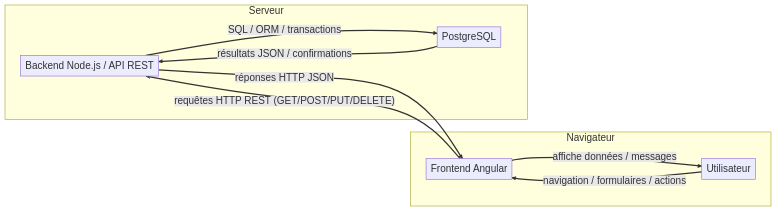
\includegraphics[width=\linewidth,height=0.75\textheight,keepaspectratio]{img/workflow_front_back_db.png}
    \caption{Workflow de communication entre l'utilisateur, le frontend, le backend et la base de données}
    \label{fig:workflow-front-back-db}
\end{figure}

\section[Déploiement et Conteneurisation : Docker]{Déploiement et Conteneurisation : Docker \raisebox{-0.2\height}{
\includegraphics[height=0.6cm]{img/logo_docker.png}}}
Afin de garantir que notre site soit "facilement installable" sur n'importe quel serveur du département informatique[cite: 14], nous avons intégré Docker dès le premier jour de développement. Docker nous permet d'encapsuler notre base de données, notre backend et notre frontend dans des conteneurs isolés. L'utilisation de \texttt{docker-compose} permet de lancer l'intégralité de l'environnement avec une seule commande, résolvant ainsi les problèmes de compatibilité entre les systèmes d'exploitation, que ce soit pour nous développeurs du projet, ou pour les futurs utilisateurs.

\section[Collaboration et Intégration Continue : GitHub]{Collaboration et Intégration Continue : GitHub \raisebox{-0.2\height}{
\includegraphics[height=0.6cm]{img/logo_github.png}}}
Travaillant en équipe de quatre, la gestion des versions du code était critique. Nous avons utilisé GitHub pour coordonner nos développements. EN plus la fusion des fonctionnalités gérée de manière fluide, GitHub nous offre le possibilitée de céeer des \textit{releases} pour le rendu final, et de créer des tickets (issues) pour répartir les tâches, de manière native.

\section{Organisation du Projet}
Afin de garantir une séparation stricte des responsabilités (separation of concerns), notre dépôt de code est structuré de la manière suivante :

\begin{verbatim}
    Gestion_locaux/
    |-- back/               # API Node.js (Logique metier et acces DB)
    |-- front/              # Application Angular (Interface utilisateur)
    |-- database/           # Fichiers SQL et scripts d'initialisation PostgreSQL
    |-- rapport/            # Sources LaTeX de ce document
    +-- docker-compose.yml  # Orchestrateur des differents conteneurs
\end{verbatim}

Cette arborescence permet à chaque membre de l'équipe de se repérer facilement et facilite le déploiement automatisé.